\chapter{Discussion}
\label{chap:Results}
\begin{figure}[ht]
    %\centering
    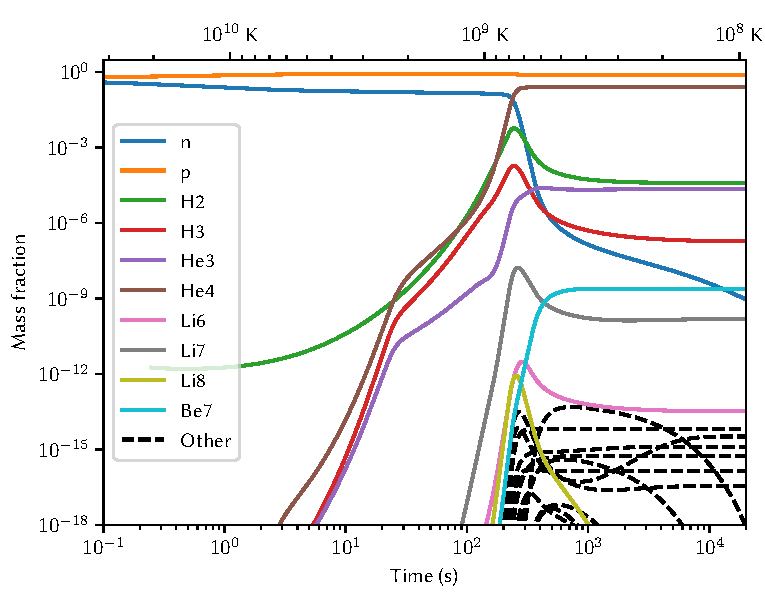
\includegraphics[width=5.1in]{figures/abundancelight.pdf}
    \caption{Time evolution of light nuclei abundance during BNN, with mass fraction technically being the close approximation $X_i=Y_i A_i$ }
    \label{fig:lightXevo}
\end{figure}
Running APODORA creates a complete overview of abundance evolution as shown on figure \ref{fig:lightXevo}. As expected neutrons protons and deuterium remain in equilibrium for the first few seconds. As the temperature decreases, deuterium abundances slowly increase quickly followed by tritium and both helium isotopes. %$2{}^2\text{H}\rightarrow {}^4\text{He}$ has a very small cross-section With ${}^4$H initially being produced primarily by ${}^3\text{H}+p\text{H}\rightarrow {}^4\text{He}$ and later by ${}^3\text{H}+{}^2\text{H}\rightarrow {}^4\text{He}+n$.
This continues until around 230 seconds, at which point the rate of ${}^4$He creation is finally great enough to have a significant impact on neutron abundance, which until then had remained almost unchanged since the $p\leftrightarrow n$ rates fell out of equilibrium. This leads to a rapid drop in neutron abundance creating a bottleneck on the production of deuterium and tritium. Without neutron capture to create more, the existing deuterium and tritium is converted to ${}^4$He via ${}^3\text{H}+{}^2\text{H}\rightarrow {}^4\text{He}+n$. Without these light nuclei lithium abundances also drop, as reactions such as ${}^4\text{He}+{}^3\text{H}\rightarrow {}^7\text{Li}$ become outmatched by the proton captures ${}^7\text{Li}+\text{p}\rightarrow 2{}^4\text{He}$ and ${}^6\text{Li}+\text{p}\rightarrow {}^7\text{Be}$. Conversely, Beryllium 7 is primarily destroyed via neutron capture ${}^7\text{Be}+\text{n}\rightarrow {}^7\text{Li}+\text{p}$, and therefore sees a rapid increase in abundance immediately after the drop in neutrons.
\begin{figure}[ht]
    %\centering
    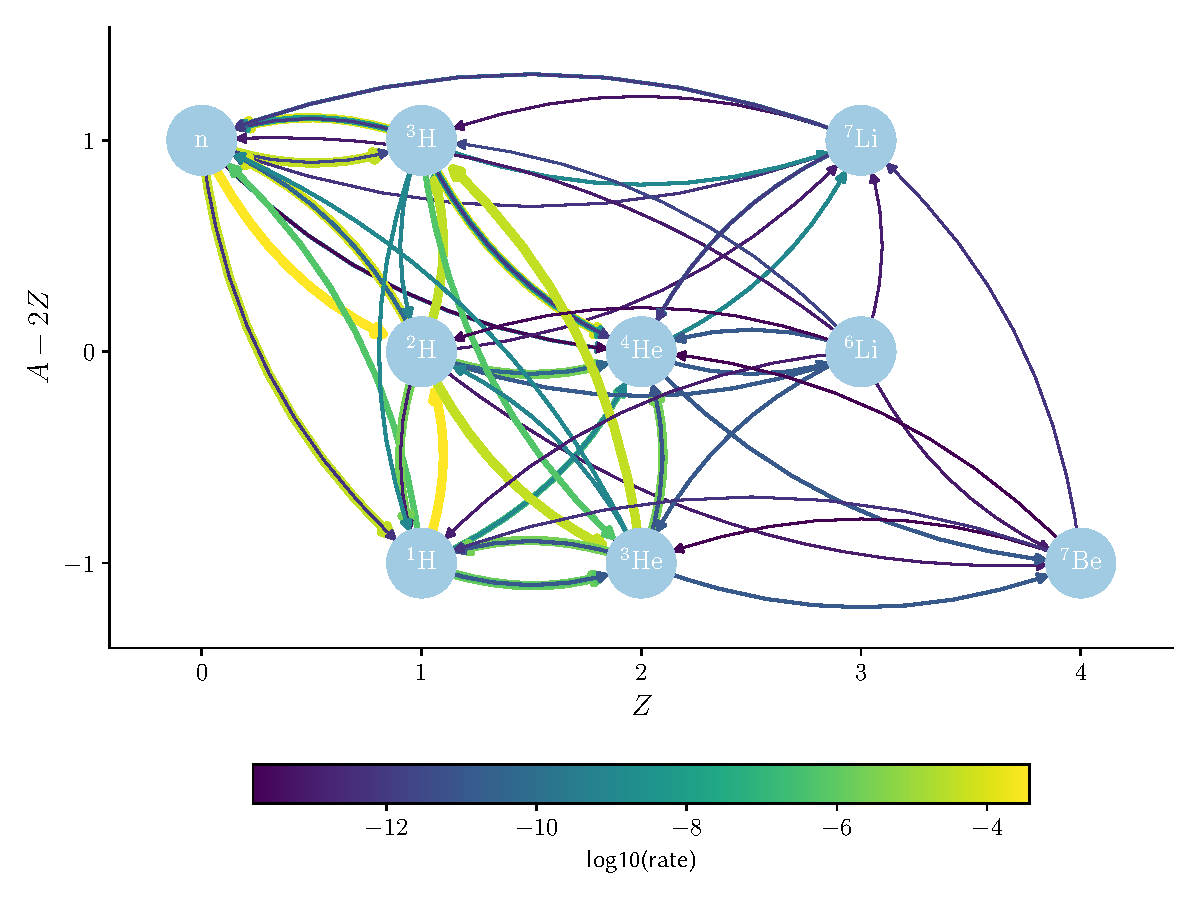
\includegraphics[width=5.1in]{figures/smallnet5minutes.pdf}
    \caption{Reaction rates 5 minutes after Big Bang at \num{7.6e8} K. Only including rates within 10 orders of magnitude of strongest. Each rate is represented by arrows from each reactant to each product}
    \label{fig:5minutenet}
\end{figure}

The relations of these reactions are illustrated in figure \ref{fig:5minutenet}. This snapshot is taken immediately after the aforementioned drop in neutron abundance with $Y_n=0.2\%$. Despite this $n+p\rightarrow d$ is still the strongest reaction rate, followed by rates creating ${}^3$He and ${}^3$H, simply due to the high abundance of these light nuclei. Though no particular reaction is exceptionally strong, a disproportionate amount of reactions produce rather than consume ${}^4$He. This should come as no surprise as ${}^4$He is the most tightly bound of all these nuclei. The only rates consuming helium are those producing heavier elements, ${}^4\text{He}+{}^3\text{H}\rightarrow {}^7\text{Li}$, ${}^4\text{He}+{}^3\text{He}\rightarrow {}^7\text{Be}$, and ${}^4\text{He}+{}^2\text{H}\rightarrow {}^6\text{Li}$. Yet these barely affect total helium abundance, and to an extent help create more ${}^4$He through subsequent reactions such as ${}^7\text{Li}+{}^2\text{H}\rightarrow 2 {}^4\text{He}+\text{n}$. 


\begin{figure}[ht]
    %\centering
    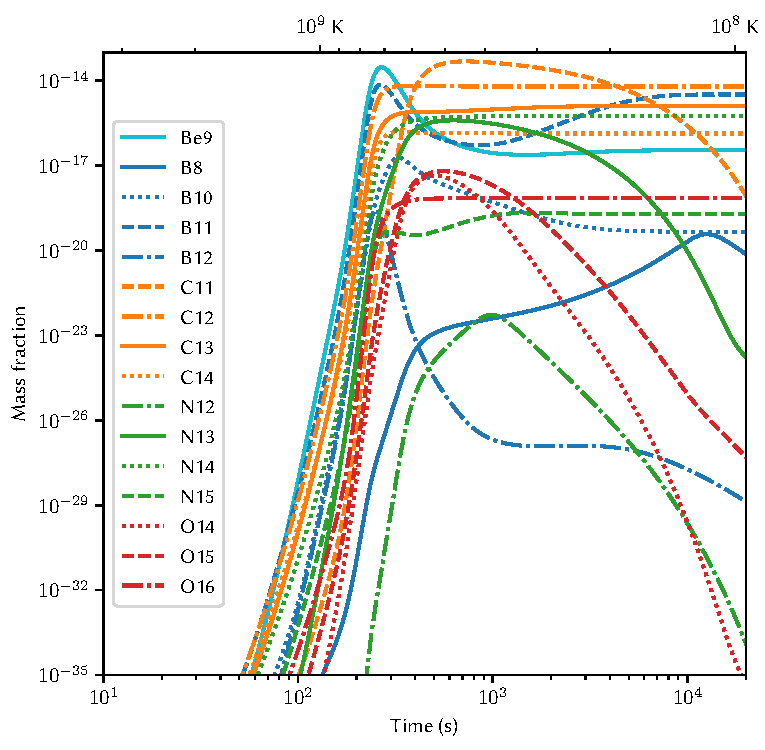
\includegraphics[width=5.1in]{figures/abundanceheavy.pdf}
    \caption{Time evolution of heavy nuclei abundance during BNN, with mass fraction technically being the close approximation $X_i=Y_i A_i$}
    \label{fig:heavyXevo}
\end{figure}

The most striking effect of the high ${}^4$He binding energy is the lack of stable nuclei with $A=8$, due 2 alpha particles being energetically favorable. Many nearby nuclei are also unstable creating a gap in the full reaction network, apparent on \ref{fig:bignet}. The next nucleus with greater binding energy per nucleon is ${}^{12}$C, which after BBN is also the most abundant of the heavy nuclei, as seen on figure \ref{fig:heavyXevo}. Bridging the gap between ${}^4$He and ${}^{12}$C is usually accomplished via the triple-alpha process $3{}^4\text{He}\rightarrow {}^{12}\text{C}$, which occurs in stars at temperatures above $10^8$K. The temperature during BBN is even higher than this, but compared to stellar interiors the density is much lower. At the previously mentioned 5 minute mark, the baryon density of the universe is only 10 grams per cubic meter, which is more than ten orders of magnitude lower than that of a helium burning stellar core. This completely stops the triple-alpha process, leaving the inefficient process of alpha capture on ${}^7$Li and later ${}^7$Be as the only options for creating heavier nuclei. This firstly creates ${}^{11}$B, which through proton capture is responsible for the majority of ${}^{12}$C production. Unfortunately the resulting exited state ${}^{12}$C* predominately decays into three alpha particles, with the branching ratio of internal translation into the ground state being only $1.5\times 10^{-4}$. The same is true for neutron capture on ${}^{11}$C, though it also decays via proton emission  ${}^{12}\text{C}^\ast \rightarrow {}^{11}\text{B}+\text{p}$ and of course freely decays ${}^{11}\text{C}\rightarrow {}^{11}\text{B}$. From figure \ref{fig:heavyXevo} we also see an initial bump in ${}^9$Be abundance caused by the uniquely high cross-section of the reaction ${}^7\text{Li}+{}^3\text{H}\rightarrow {}^9\text{Be}+n$, but as tritium abundance drops most ${}^9$Be is destroyed by photofission $\gamma+{}^9\text{Be}\rightarrow 2{}^4\text{He}+n$.


\section{Accuracy}
\label{sec:Accuracy}
Throughout the code there are several places where numerical \textbf{accuracy} must be balanced by the need for swift computation. As a baseline I aim for a relative precision on final abundances of $10^{-5}$ due to numerical uncertainty. This is much lower than the error introduced by the experimental determination of reaction rates, as well as that of astronomical observations of primordial abundances. 

\subsection{Tolerances}
For the integration itself I use the solve\_ivp method from scipy.integrate\cite{SciPy}. Here the relative and absolute tolerances must be specified as optional parameters to ensure the desired numerical accuracy. We start with the background parameters, for which only the relative tolerance matters, since the temperature and scale factor must be precise no matter their absolute value. So setting the absolute tolerance to 0 we can plot the error cause by relative tolerance.
\begin{figure}[ht]
    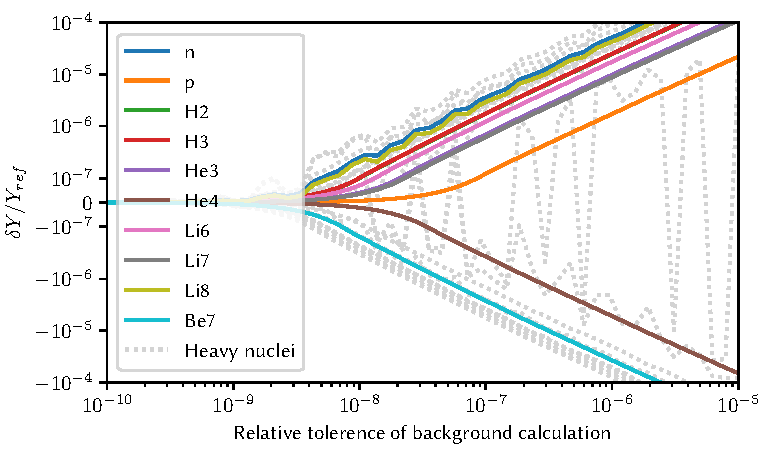
\includegraphics[width=5.1in]{figures/rtolbackground.pdf}
    \caption{Relative deviation on final abundances based on the relative tolerance used for determining background variables. Plot is linear in the region $[-10^{-7},10^{-7}]$ and logarithmic outside}
    \label{fig:rtolbackground}
\end{figure}
From figure \ref{fig:rtolbackground} it appears that the resulting error in final abundances is between one and two orders of magnitude greater than the error in background parameters. The majority of this error is not random, and seems to be caused by the lower tolerance consistently leading to a lower baryon density, as evident from the fact that ${}^{7}$Be decreases opposed to most other nuclei(\cref{fig:etaplot}). To achieve the desired accuracy of $10^{-5}$, the relative tolerance for background should be set at $10^{-7}$.

For the relative tolerance of the network, it is much more straight forward. Unsurprisingly there is a one to one correspondence between the relative tolerance and resulting error as seen on figure \ref{fig:rtolnet}. However, this is only true for the greatest outliers among the heavy nuclei. For the relevant light nuclei, the deviation is much smaller, and a relative tolerance of $10^{-4}$ should be sufficient to achieve the desired precision. 
\begin{figure}[ht]
    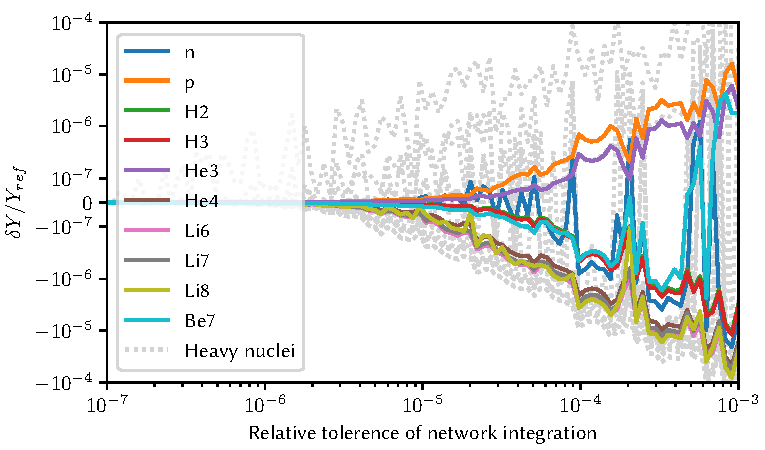
\includegraphics[width=5.1in]{figures/rtolnet.pdf}
    \caption{Relative deviation on final abundances based on the relative tolerance of the network integration. Plot is linear in the region $[-10^{-7},10^{-7}]$ and logarithmic outside}
    \label{fig:rtolnet}
\end{figure}


From figure \ref{fig:atolnet}, we see that the absolute tolerance only affect nuclei when it gets close to their final abundance. Therefore, the absolute tolerance can be set at $10^{-20}$ if accurate heavy nuclei abundance is needed, and $10^{-15}$ if only light nuclei are desired.
\begin{figure}[ht]
    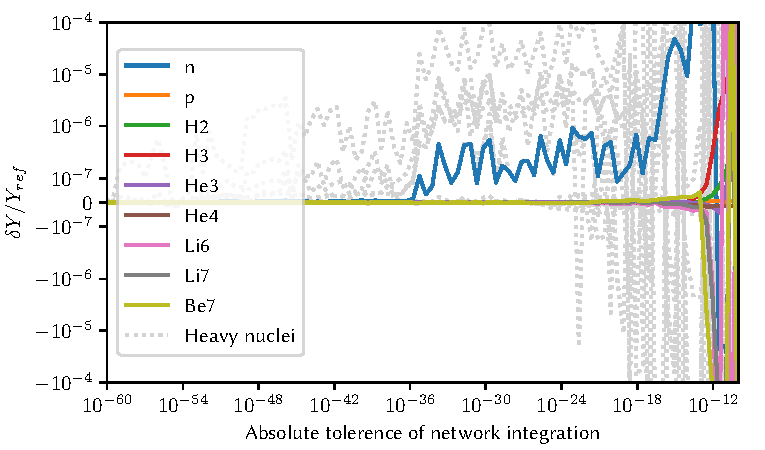
\includegraphics[width=5.1in]{figures/atolnet.pdf}
    \caption{Relative deviation on final abundances based on the absolute tolerance of the network integration. Plot is linear in the region $[-10^{-7},10^{-7}]$ and logarithmic outside}
    \label{fig:atolnet}
\end{figure}



\subsection{Electron energy}
Most calculations for the background have nice analytical expressions that can be computed with arbitrary precision. The electron energy density is the main exception, as it is given by an infinite sum \eqref{eq:rhoelectron} of which a finite number of terms must be calculated. Electrons annihilate very early, so any error in the energy density will only affect the $p\leftrightharpoons n$ rate. This will lead to a small change in neutron abundance, which results in a similar (within one order of magnitude) relative change in the abundance of all subsequent nuclei. 
Testing shows that small changes to the energy density, cause a change in neutron abundance of roughly the same relative magnitude if not slightly lower. So to achieve the requested accuracy in abundance, I also aimed for a $10^{-5}$ relative error in total energy density. 
\begin{figure}[ht!]
    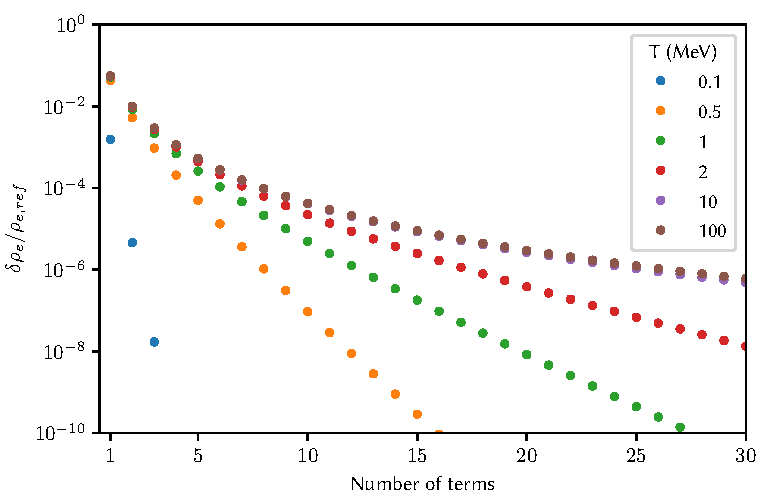
\includegraphics[width=5.1in]{figures/Besselaccuracy.pdf}
    \caption{Normalized absolute deviation of electron energy density from the reference energy as a function of included terms in \eqref{eq:rhoelectron}. The reference energy density has been determined by computing the first 10000 terms}
    \label{fig:Besselaccuracy}
\end{figure}

Figure \ref{fig:Besselaccuracy} shows the deviation from the reference energy at select temperatures before and during e$^-$ e$^+$ annihilation. For low temperatures the sum converges quickly, which should come as no surprise as the series in \eqref{eq:electronseries}, converges more rapidly as $e^{-(E\pm\mu)/T}$ approaches 0. At high temperatures the sum converges at a much slower rate, but it still achieves sufficient accuracy with only 20 terms.

\subsection{Interpolation}
\label{sec:interpolation}
For the interpolation on background variables an appropriate number of points must be selected. These points are spaced uniformly in log(t). Tests show that $10^4$ points is sufficient to achieve the required accuracy in final abundances. However, a low number of points cause the small discontinuities in the derivatives of temperature and scale factor. Due to the stiffness of the system this leads to instabilities, which have a major impact on the runtime. At the required resolution of $10^4$ the integration routine has to make twice as many call to the RHS, compared to smoother integration. At $2\times 10^5$ points the interpolations is smooth enough as to not cause issues for integration.


\subsection{Network timings}
\label{sec:networktiming}
As  mentioned in section \ref{sec:pna}, we cannot calculate the abundance of all nuclei from the beginning, and have to add them gradually as the y become relevant. To find this point we can plot the deviation in final abundance as a function of the time at which we switch between networks.
\subsubsection{Full network}
\begin{figure}[ht!]
    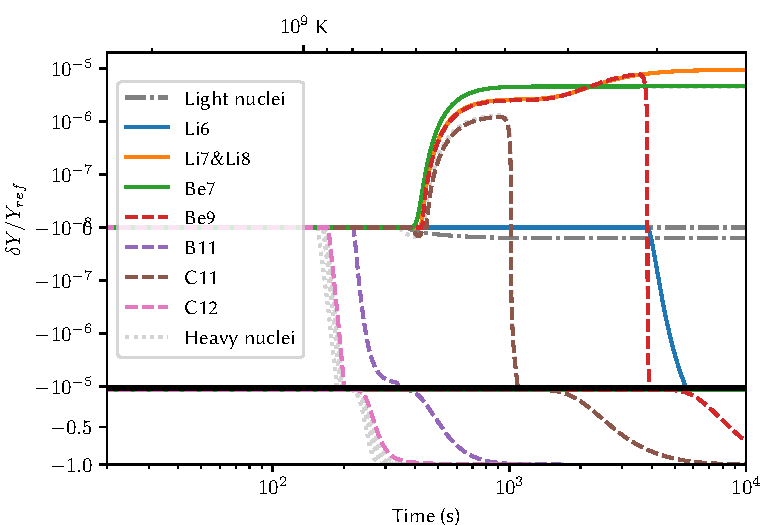
\includegraphics[width=5.1in]{figures/Bignettime.pdf}
    \caption{Relative deviation on final abundances based on the time from which heavy nuclei are included in the reaction network. To display both positive and negative changes, relative deviations $ <10^{-8}$ are excluded. The bottom shows negative deviation on a linear scale}
    \label{fig:bignettime}
\end{figure}
We start by looking at the full network shown on figure \ref{fig:bignettime}, which has three distinct points. As long as the heavy nuclei are added before the 2-minute mark corresponding to $T>10^9$K, they have time to reach the same abundance as they would if they were added earlier. Adding them later will delay the initial production, which will slowly lower the resulting final abundance. They will however still reach approximately the same final abundance until the late stages of BBN at around 7 minutes. Here the temperature will be to low for their formation, resulting in an increase in Lithium and Beryllium, as these are no longer consumed to produce heavy nuclei. 
The reaction involving ${}^{11}$C however come into effect much later than most other reactions and remain relevant even an hour after BBN. If ${}^{11}$C is added after this point, it will never achieve a significant final abundance, leading to a drop in its indirect daughter nuclei ${}^{9}$Be and ${}^{6}$Li. 

The result of this test shows that for standard BBN heavy nuclei don't actually need to be included at all, if one is only interested in abundances of light nuclei. For completeness, I will choose to include these nuclei anyway starting at $T>10^9$K. 

\subsubsection{Light network}

From figure \ref{fig:midnettime} we see that delaying the calculation of nuclear abundances, initially cause an increase abundance of protons and the proton dominated nuclei ${}^3$He and ${}^8$B, with all other abundances dropping. This is due to early nuclear reactions trapping neutrons in the cores light nuclei such as ${}^4$He and ${}^2$H, preventing their free decay into protons. However, since the vast majority of neutrons are still unbound, this effect will be insignificant until large light nuclei abundances are attained. Therefore, we actually don't need to calculate early abundances to get precise estimates of the final abundance. 

\begin{figure}[ht]
    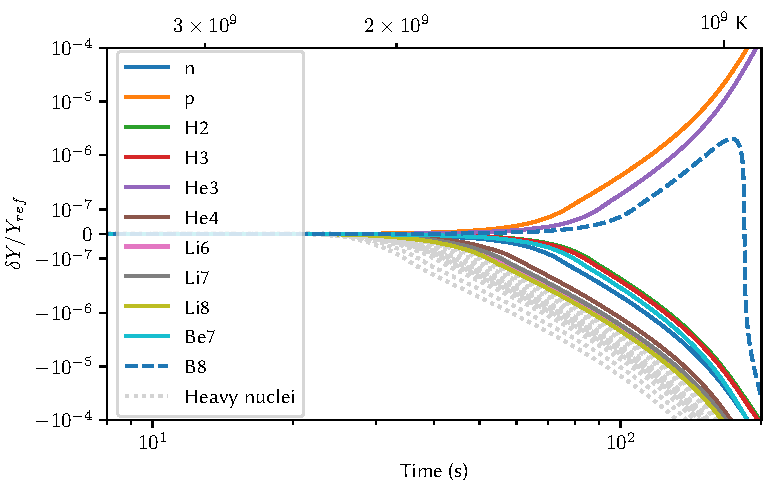
\includegraphics[width=5.1in]{figures/midnettime.pdf}
    \caption{Relative deviation on final abundances based on the time from which light nuclei are added to the reaction network. Plot is linear in the region $[-10^{-7},10^{-7}]$ and logarithmic outside}
    \label{fig:midnettime}
\end{figure}
Not having to solve the reaction network at high temperatures makes the system much less stiff, potentially allowing future BBN codes to use less complex integrations routines than those used by this and older codes. Unfortunately starting abundance calculations presents a major issue due to the initial conditions. When starting light abundance calculation at early times $t<10$s, we can determine the initial abundances by setting the RHS to 0 as described in section \ref{sec:structure}. But at later times reactions destroying ${}^4$He drop off, with ${}^4$He abundances instead being kept in check by the lack of deuterium. As the system is no longer in exact NSE, any method for determining initial condition which assume a steady state solution will fail. Given enough time all neutrons will be converted to ${}^4$He, and the estimated initial conditions reflect this by vastly overestimating ${}^4$He abundances. To get around this and produce figure \ref{fig:midnettime}, I instead had to set all initial abundances to 0 when initiating the light network after 3 seconds. This workaround eliminates the problem, but creates another in the form of transients, which are created as abundances go from 0 to their appropriate value. Since the system of equations is less stiff at these late times the transients won't break the integration. But dealing with these transients takes just as long as the time required for just tracking abundances at early times. 


\subsubsection{$p\leftrightharpoons n$ network}
Unlike the heavier nuclei the at which we start calculating neutrons and protons abundances have a very abrupt and significant impact on final abundances. As long as they are still in thermal equilibrium when we begin calculations, the final abundance will be the same. Conversely, if we start after they begin to fall out of thermal equilibrium, all final abundances will be radically different. From figure \ref{fig:npnettime} it's clear that this occurs at around 100 ms or $T=3\times10^{10}$K, and as long as we initiate $p\leftrightharpoons n$ before this we get precise results. This also justifies the use of $T=27\times10^9$K as the initial temperature, which is the point used by among others Wagoner, Kawano, and \textsc{AlterBBN}.
\begin{figure}[ht]
    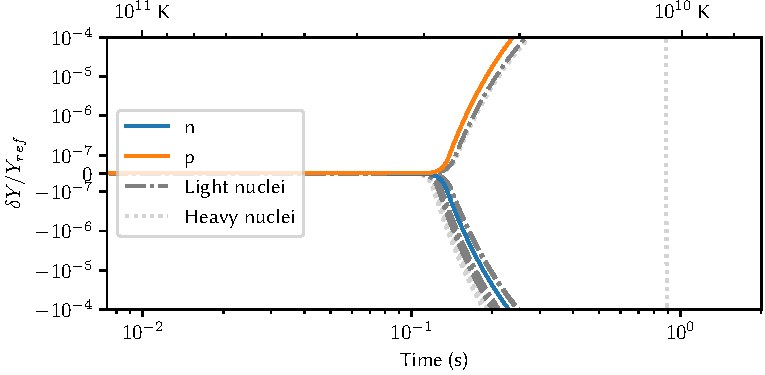
\includegraphics[width=5.1in]{figures/npnettime.pdf}
    \caption{Relative deviation of final abundances based on the initial time of BBN calculations. Plot is linear in the region $[-10^{-7},10^{-7}]$ and logarithmic outside}
    \label{fig:npnettime}
\end{figure}



\subsection{Neutrino decoupling}
\label{sec:decoupling}
The main source of inaccuracy in APODORA is the assumption of complete neutrino decoupling. This assumption is reasonable as the only net transfer of energy between different particles is annihilation of electrons and positrons, which begins at around 1 MeV as shown on figure \ref{fig:rhoegammaT}. At this point neutrinos have mostly  decoupled, and therefore the energy is transferred to the photons, which are heated relative to the neutrinos by the well known factor $\sqrt[3]{11/4}$. There is however a small transfer of energy before the neutrinos completely decouple from the other particles. The result of this is a small increase in neutrino energy density relative to photon energy of around 1\% \cite{Hannestad:1995rs}. As both neutrinos and photons are ultrarelativistic, this change is inconsequential to the time evolution of the early universe, and therefore one might assume that it would not have a significant impact on final abundances. This is however not the case, as is apparent from figure \ref{fig:initime}. The reason for this is that the higher photon temperature caused by instantaneous decoupling, effectively delays the onset of nucleosynthesis, since the baryons take longer to cool sufficiently. This has two main effects, the first being slightly lower baryon density at any given temperature, and the second that the universe will remain in any given temperature range for longer. Additionally, neutrino decoupling also affects the $p\leftrightharpoons n$ reactions directly, as these rely on both exact temperature and non-thermal energy distribution of the neutrinos. When assuming complete neutrino decoupling, these effects lowers the abundance of ${}^4$He by 0.05\%, ${}^3$He by 0.1\%, and deuterium by 0.5\%, and increase ${}^7$Be by 0.5\%, (PRIMAT table V\cite{PRIMAT}). 

As mentioned in section \ref{sec:rhoNeutrino}, we can compensate for this by using an effective neutrino number $N_\nu^\text{eff}=3.045$, to account for the transferred energy. Yet, this was implemented when producing figure \ref{fig:initime}, which still show deviations characteristic of an altered $T_\nu/T_\gamma$ ratio. This is due to $N_\nu^\text{eff}$ effectively adding additional energy to the universe, which causes the universe to expand more rapidly, cooling the neutrinos. Secondly the electrons and positrons are not completely relativistic, which causes the temperature of coupled components to not scale exactly with $a^{-4}$. To reduce the deviation in $T_\nu/T_\gamma$ ratio, we can decouple the neutrinos as close as possible to the point at which they actually decouple. This still assumes an instant rather than gradual decoupling, but nonetheless improves predicted abundances. The point at which neutrinos decouple obviously coincide with the freezeout of $p\leftrightharpoons n$ reactions, and as shown on \ref{fig:npnettime}, we can safely begin both background and network integration at 27 GK corresponding to 2.3 MeV. 
\begin{table}[ht]
    \begin{tabular}{l|llllll}
        & $Y_p \times 10$ & \hspace{-0.34em}$^{2}$H$ \times 10^{5}$ & \hspace{-0.34em}$^{3}$He$ \times 10^{5}$ & \hspace{-0.34em}$^{7}$Li $ \times 10^{10}$& \hspace{-0.34em}$^{6}$Li $ \times 10^{15}$& \hspace{-0.34em}$^{7}$Be $ \times 10^{10}$\\ \hline
    100 MeV & 2.470            & 2.532 & 1.040 & 4.712 & 7.503 & 4.411     \\ \hline
    2.3 MeV  & 2.472            & 2.536 & 1.040 & 4.706 & 7.523 & 4.404   \\ \hline
    Deviation & 0.07\%           & 0.15\% & 0.04\% & -0.15\% & 0.25\% & -0.18\%      
    \end{tabular}
    \caption{Comparison of final abundances for instant decoupling at 2.3 and 10 MeV, with all abundances except ${}^4$He ($Y_p$) being normalized to H abundance. ${}^3$He and ${}^7$Li including contribution from eventual decay of ${}^3$H and ${}^7$Be}
    \label{tab:earlylatedecoup}
\end{table}
From table \ref{tab:earlylatedecoup} we clearly see the impact of neutrino decoupling. Compared to the expected changes determined by PRIMAT\cite{PRIMAT}, we see an increased impact on ${}^4$He and a reduced impact on ${}^7$Be and ${}^3$He. This can mostly be explained by the $p\leftrightharpoons n$ reactions not being directly impacted in my implementation. The direct effect on $p\leftrightharpoons n$ increases the neutron abundance and subsequently the abundance of all other nuclei, counteracting the effects on everything but ${}^7$Be, as well as ${}^3$He since its abundance actually increases as neutron abundance drops.%The direct effect only changes the neutron proton ratio, which partially cancels the changes introduced by the delay of nucleosynthesis, particularly in ${}^4$He abundance. Therefore, the theoretical systematic error in ${}^4$He is slightly higher, which we will explore further in section \ref{sec:Altercompare}.
\begin{figure}[ht]
    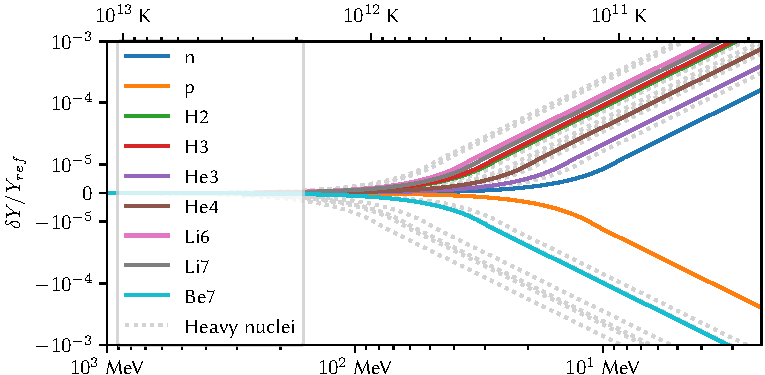
\includegraphics[width=5.1in]{figures/initime.pdf}
    \caption{Relative deviation on final abundances based on the initial time for background calculations. By construction the initial time coincides with the time of neutrino decoupling}
    \label{fig:initime}
\end{figure}

Though the errors associated with neutrino decoupling are much greater than the achieved numerical error of less than $10^{-5}$, they are still acceptable, since they are completely inconsequential next to the uncertainty associated with reactions rates, as will become apparent in the following section.


\section{Comparison with AlterBBN}
\label{sec:Altercompare}
To compare the results of APODORA to that of other contemporary BBN codes, I have chosen \textsc{AlterBBN}. The main reason for this is that it is more accessible, with the code being directly available on GitHub, while not requiring a Mathematica license like PRIMAT. Additionally, both APODORA and \textsc{AlterBBN} uses natural units for the background calculations and cgs units for the reaction network. This makes direct comparison of numerical values easier as the only conversion required is an occasional factor of $10^3$, due to the energy being measured in GeV rather than MeV.%PArthENoPE would also be a fine choice, but since it doesn't explicitly track time


\subsection{Speed}
As \textsc{AlterBBN} is written purely in C, it unsurprisingly runs faster than my Python implementation, despite the "outsourcing" of the reaction network. Using WSL and GCC-11.3 on an Intel i3-1115G4 @ 3.00GHz, I get an average runtime of 0.61 seconds, of which 0.33 seconds are for the background calculation, and 0.28 seconds for the network integration. This is slightly slower than the 0.38 seconds for the default routine of \textsc{AlterBBN}. However, the integration method of \textsc{AlterBBN} sacrifices accuracy for speed, with the default method causing numerical deviation on final abundances of up to 0.4\%. \textsc{AlterBBN} can employ alternate methods for more accurate results, but these have a major impact on runtime. To achieve the same numerical accuracy as this implementation, we must use the most precise integration method in \textsc{AlterBBN} which takes 53.91 seconds. So if numerical consistency above $10^{-3}$ is required, this implementation is much faster, despite being implemented in Python rather than C.  Based on this, the requirement of \textbf{Alacrity} has been fulfilled.

\subsection{Predicted abundances}
\begin{table}[ht]
    \begin{tabular}{l|llllll}
        & $Y_p \times 10$ & \hspace{-0.34em}$^{2}$H$ \times 10^{5}$ & \hspace{-0.34em}$^{3}$He$ \times 10^{5}$ & \hspace{-0.34em}$^{7}$Li $ \times 10^{10}$& \hspace{-0.34em}$^{6}$Li $ \times 10^{14}$& \hspace{-0.34em}$^{7}$Be $ \times 10^{10}$\\ \hline
    APODORA & 2.472            & 2.536 & 1.040 & 4.706 & 0.752 & 4.404   \\ \hline
    \textsc{AlterBBN} & 2.474            & 2.467 & 1.034 & 5.363 & 1.087 & 5.075   \\ %\hline
    $\quad +/-$ & 0.003           & 0.038 & 0.016 & 0.352 & 1.085 & 0.343      
    \end{tabular}
    \caption{Abundances from APODORA and \textsc{AlterBBN}, with all abundances except ${}^4$He ($Y_p$) being normalized to the H abundance. ${}^3$He and ${}^7$Li including contribution from eventual decay of ${}^3$H and ${}^7$Be. Quoted uncertainties are those determined by \textsc{AlterBBN}}
    \label{tab:shortAlterabun}
\end{table}
Comparing the final abundances predicted by APODORA and \textsc{AlterBBN} we see major discrepancies. Most of these are within the uncertainties calculated by \textsc{AlterBBN} based on the uncertainty of the reaction rates. ${}^7$Be and subsequently ${}^7$Li deviate by more than twice what is predicted, and the same is true for deuterium. To discover the cause of this we can do a 1 to 1 comparison of the time evolution of the universe according to APODORA and \textsc{AlterBBN}. Here we use the exact same initial conditions of $T=27\times10^9$K, $\eta=6.1\times 10^{-10}$ and $\tau_n=880.2$s, remembering to correct for the inaccurate initial time in \textsc{AlterBBN} as explained in section \ref{sec:t_ini}.

\subsection{Background}
\label{sec:AlterBackground}
To rule out cosmological differences, we can compare the predicted background parameters from \textsc{AlterBBN} and APODORA, displayed on figure \ref{fig:comparetemp}. Unsurprisingly after the common initial temperature of 27GK, \textsc{AlterBBN} sees a relative increase in neutrino temperature due to incomplete neutrino decoupling. The photon temperature initially decreasing more slowly, since this term is identical for both codes. But this will also begin to slowly drop, due to the difference in energy transfer. Later there is a small additional drop in photon temperature coinciding with the onset of primary nucleosynthesis. This can be explained by \textsc{AlterBBN} taking into account the effect of nucleosynthesis on photon temperature, due to the energy release of nucleosynthesis. However, the observed effect is unphysical and must be due to numerical errors, since the energy release is nowhere near the amount required for an impact on photon temperature of this size, and additionally it should serve to increase, rather than decrease the photon temperature. Lastly, there is a relative decrease of the \textsc{AlterBBN} neutrino temperature at late times. This is due to \textsc{AlterBBN} taking into account both baryon and dark matter energy density, which I have omitted since it clearly doesn't have a significant impact during the era of BBN.
\begin{figure}[ht]
    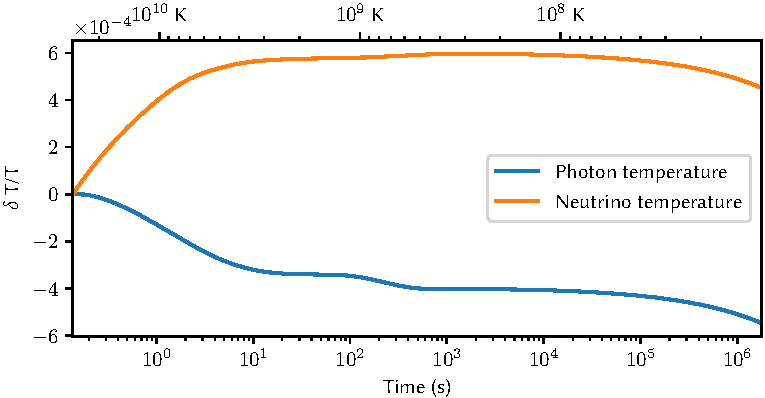
\includegraphics[width=5.1in]{figures/comparetemp.pdf}
    \caption{Relative deviation of temperatures as calculated by APODORA and \textsc{AlterBBN}. Positive values signify higher \textsc{AlterBBN} temperatures compared to APODORA}
    \label{fig:comparetemp}
\end{figure}

\noindent To see the impact of these background differences we can integrate the reaction network using the background parameters from \textsc{AlterBBN}. At its highest precision setting \textsc{AlterBBN} takes 64421 discreet time steps, which based on the test in section \ref{sec:interpolation} is sufficient to achieve high accuracy with the existing interpolation routine. \textsc{AlterBBN} does however not directly track the scale factor, so we must instead track the baryon density using the neutrino temperature. Since the tabulated $p\leftrightharpoons n$ rates used in this network only depend on temperature, we don't need to know the exact value of $n_b$ before the other reactions become relevant at around 100 seconds, (figure \ref{fig:midnettime}). At this time neutrinos have actually decoupled completely, and therefore the relation $T_\nu \propto a^{-1}$ holds exactly. This allows the baryon number density to be determined by $n_b= C \cdot T_\nu^3$ with the constant $C$ being set by requiring $\eta=6.1\times 10^{-10}$ at late times.
\begin{table}[ht]
    \begin{tabular}{l|llllll}
               & $Y_p \times 10$ & \hspace{-0.34em}$^{2}$H$ \times 10^{5}$ & \hspace{-0.34em}$^{3}$He$ \times 10^{5}$ & \hspace{-0.34em}$^{7}$Li $ \times 10^{10}$& \hspace{-0.34em}$^{6}$Li $ \times 10^{14}$& \hspace{-0.34em}$^{7}$Be $ \times 10^{10}$\\ \hline
    100 MeV & 2.470            & 2.532 & 1.040 & 4.712 & 0.750 & 4.411     \\ \hline
    2.3 MeV  & 2.472            & 2.536 & 1.040 & 4.706 & 0.752 & 4.404    \\ \hline
    \begin{tabular}[c]{@{}l@{}}APODORA using \\ \textsc{AlterBBN} $T_\gamma$ \& $T_\nu$ \end{tabular} & 2.473            & 2.540 & 1.041 & 4.699 & 0.754 & 4.398   \\ \hline
    \textsc{AlterBBN} & 2.474            & 2.467 & 1.034 & 5.363 & 1.087 & 5.075   \\ %\hline
    $\quad +/-$ & 0.003           & 0.038 & 0.016 & 0.352 & 1.085 & 0.343     
    \end{tabular}
    \caption{Comparison of final abundances for various background parameters. Showing results of this network using early and late instant neutrino decoupling, as well as the \textsc{AlterBBN} background which accounts for incomplete decoupling. The last row shows result from the \textsc{AlterBBN} background using their own abundance calculations}
    \label{tab:longAlterabun}
\end{table}

The result of using the background parameters of \textsc{AlterBBN} are displayed in Table \ref{tab:longAlterabun}. Though somewhat obscured by the lack of significant digits, relative change caused by using the \textsc{AlterBBN} background is equal to 90\% of the change caused by changing the timing of instant neutrino decoupling. This is due to the increase in $T_\nu/T_\gamma$ predicted by full incomplete decoupling, being 1.9 times greater than what is achieved by simply delaying instant decoupling. ${}^4$He however only increases by 68\% of that caused by delayed decoupling. This is due to ${}^4$He being governed by the $p\leftrightharpoons n$ reactions, which take place while $T_\nu/T_\gamma$ is still increasing. This supports the previous assumption, that the only major difference between the cosmological calculation of \textsc{AlterBBN} and APODORA, is their inclusion of incomplete neutrino decoupling.

\subsection{Reaction network}

Since the difference in background introduces minimal abundance corrections, the discrepancy between the \textsc{AlterBBN} results and mine must unsurprisingly be due to differences in the reaction network. To see where these differences are we can plot the relative difference between abundances as they evolve during BBN, displayed on figure \ref{fig:AlterBBNdeltaY}. 
\begin{figure}[ht]
    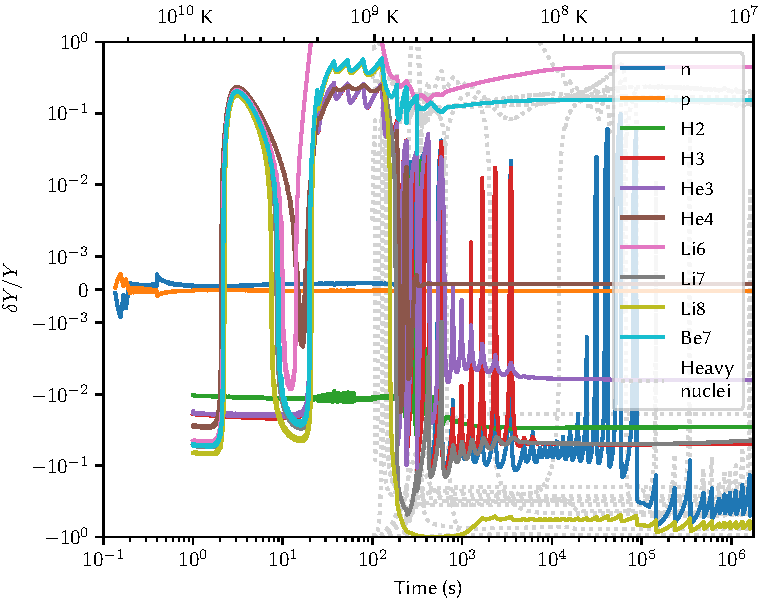
\includegraphics[width=5.1in]{figures/AlterBBNdeltaY.pdf}
    \caption{Relative deviation on abundances between APODORA and \textsc{AlterBBN}, during the various stages of BBN. To rule out cosmological differences, the \textsc{AlterBBN} background parameters are used for both calculations. Plot is linear in the region $[-10^{-3},10^{-3}]$ and logarithmic outside}
    \label{fig:AlterBBNdeltaY}
\end{figure}


Starting at the high temperature limit, we see how the differences in early $p\leftrightharpoons n$ rates cause a deviation in proton and neutron abundance. This deviation corresponds exactly to that of the final ${}^4$He abundance. We can therefore conclude that the difference in $Y_p$ is purely due to differences in this rate. 

The next notable difference is the relative increase and subsequent drop in ${}^4\text{He}$ abundances, which takes place between 2 and 20 seconds. This matches the time period where in which the relative strength of the ${}^3\text{He}+n\rightarrow {}^4\text{He}$ rate is greatest compared to that of other reactions for ${}^4$He production. Suspecting this particular reaction is further supported by \textsc{AlterBBN} using a linear approximation for the rate, stemming from the original Wagoner code\cite{Wagoner69}. Though inaccurate, this doesn't actually have a significant impact on final abundances since the reaction only dominates ${}^4\text{He}$ production at very early times. 

Following this we see the most striking feature, which are the periodic spikes in relative abundance affecting almost every single nuclei. This jaggedness originates in \textsc{AlterBBN}, and is caused by their implementation of certain reaction rates. As described in section \ref{sec:pna}, I use smooth fits of experimental data to obtain appropriate values for the reaction rates at any temperature. With every one of these rates stemming from the most recent snapshot of the REACLIB database\cite{REACLIB} available in pynucastro\cite{pynucastro2}. \textsc{AlterBBN} on the other hand uses a manually curated list of reaction rates, with a myriad of different sources and implementations. A few of these rates are tabulated, and to obtain values between the tabulated temperature steps, \textsc{AlterBBN} simply uses nearest neighbor interpolation. This is hard coded as a series of consecutive else/if statements, which return the value of the reaction rate in discreet steps according to the nearest tabulated value. The spikes happen whenever these rates assume a new value. As an example \textsc{AlterBBN} uses a tabulated ${}^2\text{H}+p\rightarrow {}^3\text{He}$ rate from \textcite{Coc_et_al_2015}, which is responsible for the small early spikes in ${}^3\text{He}$, and other nuclei that depend on its abundance. This can be confirmed by noting that the early spikes peak at 1.875, 1.625, 1.375, and 1.125 GK, which happen to be the exact midpoints between the tabulated values which are at 2, 1.75, 1.50, 1.25, and 1 GK. 


These spikes obscure what processes responsible for the deviation in nuclear abundances, but for ${}^7\text{Li}$ and ${}^7\text{Be}$ in particular we can make very good guesses as to what these reactions are. The primary reactions responsible for creating and destroying ${}^7\text{Li}$ are ${}^3\text{H}+{}^4\text{He}\rightarrow {}^7\text{Li}$ and ${}^7\text{Li} + p\rightarrow 2{}^4\text{He}$, with ${}^7\text{Be}$ being governed by ${}^3\text{He}+{}^4\text{He}\rightarrow {}^7\text{Be}$ and ${}^7\text{Be} + n\rightarrow {}^7\text{Li} + p$. Compared to these, all other reactions are completely insignificant, which can be seen on \cref{fig:Be7destruct,fig:Be7create,fig:Li7destruct,fig:Li7create}. This makes these reactions the most likely cause of the deviations, which is further supported by \textsc{AlterBBN} and my network using different rates for each one of these them.

\subsection[Modifying the Network with AlterBBN rates]{Modifying the Network with AlterBBN rates}

To test these claims we can replace the default rates in my network with the four ${}^7\text{Li}$ and ${}^7\text{Be}$ rates from \textsc{AlterBBN} as well as the previously mentioned ${}^3\text{He}+n\rightarrow {}^4\text{He}$ rate. Due to the modular nature of my reaction network this is quite easy to accomplish, with the resulting abundances being shown on \cref{tab:Alterratesabun}.
\begin{table}[ht]
    \begin{tabular}{l|llllll}
               & $Y_p \times 10$ & \hspace{-0.34em}$^{2}$H$ \times 10^{5}$ & \hspace{-0.34em}$^{3}$He$ \times 10^{5}$ & \hspace{-0.34em}$^{7}$Li $ \times 10^{10}$& \hspace{-0.34em}$^{6}$Li $ \times 10^{14}$& \hspace{-0.34em}$^{7}$Be $ \times 10^{10}$\\ \hline
    Default rates  & 2.473    & 2.540 & 1.041 & 4.699 & 0.754 & 4.398    \\ \hline
    \begin{tabular}[c]{@{}l@{}}Rates from  \\ \textsc{AlterBBN} \end{tabular} & 2.473    & 2.540 & 1.041 & 5.133 & 0.754 & 4.837    \\ \hline
    \textsc{AlterBBN} & 2.474            & 2.467 & 1.034 & 5.363 & 1.087 & 5.075   \\ %\hline
    $\quad +/-$ & 0.003           & 0.038 & 0.016 & 0.352 & 1.085 & 0.343     
    \end{tabular}
    \caption{Final abundances for the default APODORA network, the network using select \textsc{AlterBBN} rates, and the results from \textsc{AlterBBN}}
    \label{tab:Alterratesabun}
\end{table}
As expected only the abundances of ${}^7\text{Li}$ and ${}^7\text{Be}$ are affected, since the total abundances of light nuclei involved in the four reactions are much higher. 

Though the modified rates bring ${}^7\text{Li}$ and ${}^7\text{Be}$ abundances within the estimated uncertainty of \textsc{AlterBBN}, they still deviate significantly. To explain this figure \ref{fig:AlterBBNdeltaY} can be recreated using the modified reaction network, resulting in figure \ref{fig:AlterratesBBNdeltaY}. Looking at the early abundances we confirm that the initial difference in light nuclei abundance was indeed caused by the ${}^3\text{He}+n\rightarrow {}^4\text{He}$ rate. Additionally, we see how the spiking affects both ${}^7\text{Li}$ and ${}^7\text{Be}$ right up until the point at which they settle into their final abundances, making this the most likely explanation for the remaining discrepancy.

\begin{figure}[ht]
    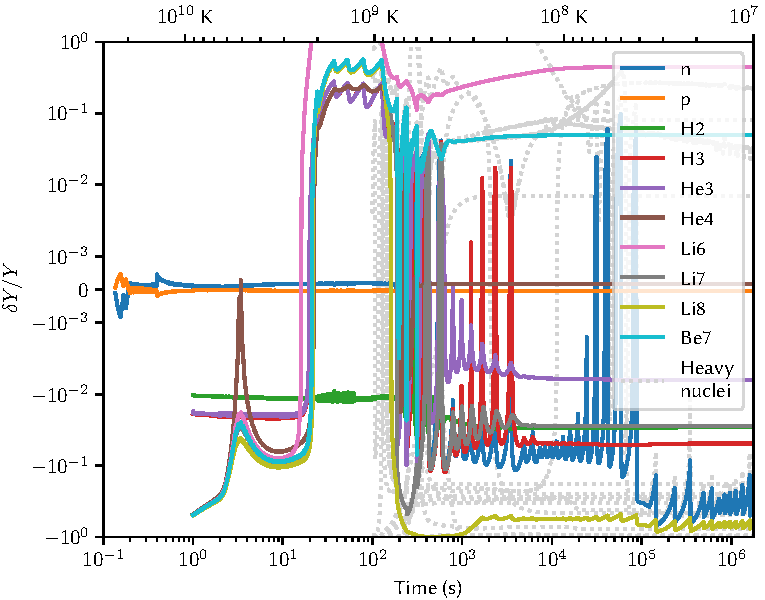
\includegraphics[width=5.1in]{figures/AlterratesBBNdeltaY.pdf}
    \caption{Same as \cref{fig:AlterBBNdeltaY}, but with the network using the same rates as \textsc{AlterBBN} for the reactions ${}^3\text{He}+n\rightarrow {}^4\text{He}$, ${}^7\text{Li}$ are ${}^3\text{H}+{}^4\text{He}\rightarrow {}^7\text{Li}$, ${}^7\text{Li} + p\rightarrow 2{}^4\text{He}$, ${}^3\text{He}+{}^4\text{He}\rightarrow {}^7\text{Be}$, and ${}^7\text{Be} + n\rightarrow {}^7\text{Li} + p$}
    \label{fig:AlterratesBBNdeltaY}
\end{figure}



\section{Final abundances}

With differences between APODORA and \textsc{AlterBBN} established, we can look at the correlation with the other codes, and more importantly the actual observations. 
\begin{table}[ht]
    \begin{tabular}{l|llllll}
               & $Y_p \times 10$ & \hspace{-0.34em}$^{2}$H$ \times 10^{5}$ & \hspace{-0.34em}$^{3}$He$ \times 10^{5}$ & \hspace{-0.34em}$^{7}$Li $ \times 10^{10}$\\ \hline
    Observations  & 2.453$\pm$0.034    & 2.527$\pm$0.030 & <1.1$\pm$0.2 & 1.6$\pm$0.3    \\ \hline
    APODORA  & 2.472            & 2.536 & 1.040 & 4.706     \\ \hline
    \textsc{AlterBBN} & 2.474$\pm$0.003 & 2.467$\pm$0.038 & 1.034$\pm$0.016 & 5.363$\pm$0.343    \\ \hline
    PRIMAT & 2.4709$\pm$0.0017   & 2.459$\pm$0.036 & 1.074$\pm$0.026 & 5.623$\pm$0.247   \\ \hline
    PArthENoPE& 2.4687$\pm$0.0012     & 2.51$\pm$0.06 & 1.032  & 4.688      
    \end{tabular}
    \caption{Observed final abundances\cite{Yp_Aver_2021}\cite{deuterium_Cooke_2018}\cite{Allobsabun}, and the predictions by various BBN codes\cite{AlterBBN}\cite{PRIMAT}\cite{PArthENoPE},}
    \label{tab:Obsabun}
\end{table}
From \cref{tab:Obsabun}, we see how the abundances predicted by APODORA lie within the span of the values obtained by other codes. 

\subsubsection{Y$_\textbf{p}$}
PRIMAT and PArthENoPE both have very precise estimates for $Y_p$ which are mutually consistent. This is due to them both calculating the exact $p\leftrightharpoons n$ rates with very high precision. I get a slightly higher estimate, which is primarily due to the lack of incomplete neutrino decoupling, and that unlike PRIMAT and PArthENoPE, the $n \leftrightharpoons p$ rate I use doesn't include bremsstrahlung corrections\cite{Serpico_2004}. The effect of these corrections are given in \textcite[table V]{PRIMAT}, as $\delta Y_p = 1.2\times10^{-4}$ and $\delta Y_p = -3.1\times10^{-4}$. If we correct for this we get a final abundance of $Y_p\times 10 = 2.4721+0.0012-0.0031=2.4702$, which is consistent with both PRIMAT and PArthENoPE.

\subsubsection{$^\textbf{2}$H}
Deuterium stands out with, my implementation being outside the quoted uncertainty of both \textsc{AlterBBN} and PRIMAT. As always this is most likely due to a different choice of reaction rates. In particular the rate for ${}^2\text{H}+n\rightarrow {}^3\text{He}$, for which REACLIB uses a theoretical rate from \textcite{Reaclibdphe3_2004}, as opposed to the other codes which use more recent experimental rates. For \textsc{AlterBBN} and the 2018 snapshot of PRIMAT, this results in lower deuterium abundances. Yet it matches PArthENoPE since they use a recent rate from LUNA, which is actually closer the old theoretical rate than previous experimental rates\cite{Luna_impact_Pisanti_2021}. 

\subsubsection{$^\textbf{3}$He}
For $^{3}$He my results match those of \textsc{AlterBBN} and PArthENoPE, with PRIMAT being slightly higher. Different reaction rates might explain this difference, but due to the poor observational constraints this is not a major issue. 

\subsubsection{$^\textbf{7}$Li}
${}^7\text{Li}$ is where we see the largest deviation. Relative to \textsc{AlterBBN} we know this is due to different reactions rates, and this is also the most probable explanation for PRIMAT. PArthENoPE once again shows better agreement, since they in this case use many of the same reaction rates as those in REACLIB. There is still a small difference which is likely to be caused by the lack of incomplete decoupling. Yet compared to the difference caused by different rates in PRIMAT and \textsc{AlterBBN}, this is completely inconsequential, which once again justifies the omission of incomplete decoupling. Yet, every single code is still nowhere near the observational value, which is of course the infamous cosmological lithium problem.


\subsection[eta and the Lithium problem]{$\eta$ and the Lithium problem}
The most well known illustration of the lithium problem is obtained by plotting the final abundances as a function of primary free parameter of BBN $\eta$. At any specific time the balance of various reaction rates is determined by the ratio of baryon density and temperature. Barring radically different physics, any cosmological solution to the lithium problem will involve modifying this ratio, for which $\eta$ is a direct proxy. Since the REACLIB rates don't include the associated uncertainties, I am unable to make a direct estimate of the uncertainty of my results. However, since these uncertainties stem from the same reactions as those in other codes, I can use an average of these to get a reasonable upper bound on the uncertainty. Additionally, the predicted uncertainties of other codes are demonstrably too conservative. For figure \ref{fig:etaplot}, the estimated uncertainties used are $ Y_p=0.1\%$, $^{2}$H=2\%, $^{3}$He=2\%, and $^{7}$Li=8\%.

\begin{figure}[ht]
    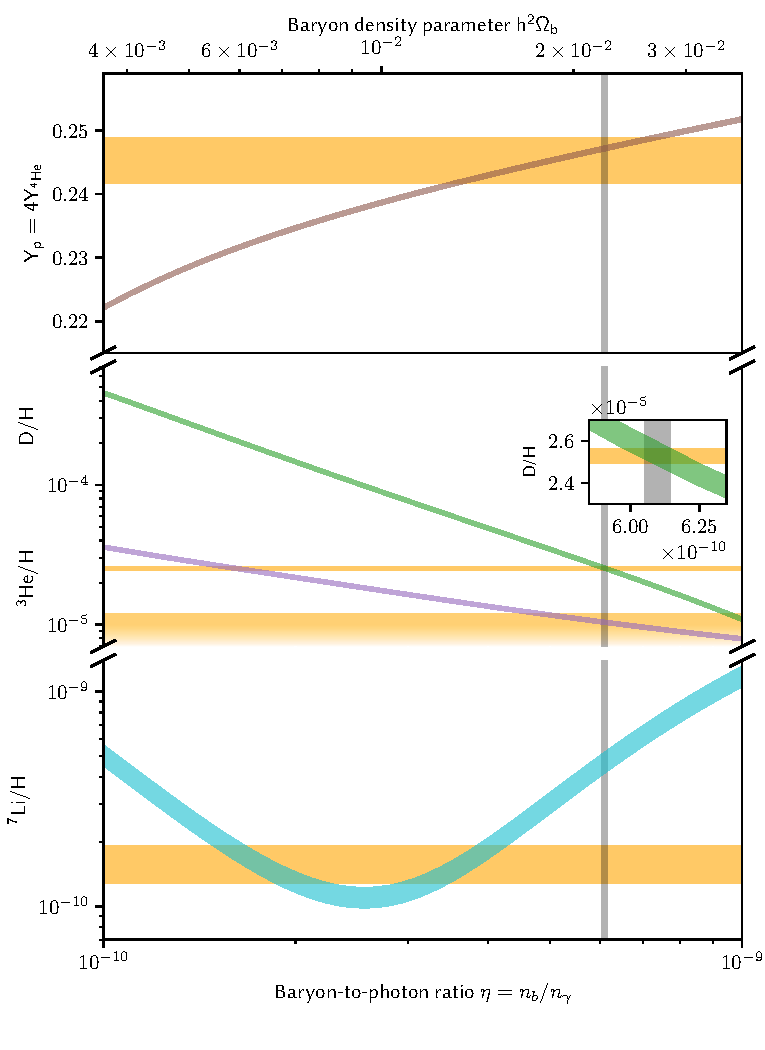
\includegraphics[width=5.1in]{figures/etaplot.pdf}
    \caption{Resulting final abundances for different values of $\eta$. Gray lines represent the value for $\eta$ from the most recent Planck results\cite{Planck}. Orange represent the observational constraints given in \cref{tab:Obsabun}. The remaining lines are the abundances produced by APODORA, with uncertainties estimated based on those of comparable networks}
    \label{fig:etaplot}
\end{figure}
%\section{Nuclear solutions to the Lithium problem?}

We see how my results match the expected abundances for all observable nuclei except lithium. We also see how any cosmological solution to this problem would inevitably lead to an even worse "deuterium problem". 
\clearpage
\section{Outlook}

The flexibility of APODORA will allow for easier investigations into the physical processes of BBN, especially nuclear processes. 

One such use would be to systematically identify the relevant reactions for BBN. With the pynucastro interface we can easily evaluate the different reaction rates, without having to modify the actual BBN calculations. I previously used this to create the plots in \cref{chap:more_plots}, and identify the primary rates mentions in the beginning of \cref{chap:Results}. This could be extended to create a new reaction network, without the countless rates that don't significantly impact final abundances, which would be very useful, as the number of reaction rates that must be evaluated, is one of the main factors increasing runtime. More importantly, systematically identifying these rates would be useful not only to this, but every single BBN code. 

To further improve speed at the cost of accessibility, the solution methods in APODORA could be implemented in a compiled language such as C and C++. This has the potential to be one of, if not the fastest BBN code currently available. Most of the required calculations are quite simple and would be easy to implement, with the main exceptions being the modified Bessel functions and the Radau IIA integration method. These however are well known and have many existing implementations\cite{C_Bessel}. For the reaction network pynucastro supports generating the network in both Python and C++. 

A C/C++ version of APODORA would also be very useful for interfacing directly with CLASS\cite{CLASS_Diego_Blas_2011}. The Cosmic Linear Anisotropy Solving System is a Boltzmann code, which calculates the theoretical power spectrum based on cosmological parameters. The ability to also make predictions on BBN abundances, would be an excellent way to provide additional constrains when testing cosmological models. Among the various available Boltzmann codes CLASS is an obvious choice, as its stated goals of user-friendliness, flexibility, accuracy and speed\cite{CLASS_Diego_Blas_2011}, are the same as those of this BBN code. But of course the primary reason for integrating APODORA with CLASS, is that my supervisor is one of the main developers. 

Another use would be to compare the background calculation of various BBN non-BBN codes, as was done with \textsc{AlterBBN} in section \ref{sec:AlterBackground}. This is only possible due to APODORA completely separating the calculation of background parameters and nuclear processes. The modular structure could even lead to multiple unique codes for calculating either the background or the reaction network. This would make it much easier to compare BBN codes, as it would definitively identify what or if differences are cosmological or nuclear in origin. 

%The next step for this project will be further optimization of the code. 

%The Cosmic Linear Anisotropy Solving System (CLASS) is a new accurate Boltzmann code, designed to offer a more user-friendly and flexible coding environment to cosmologists. CLASS is very structured, easy to modify, and offers a rigorous way to control the accuracy of output quantities. It is also incidentally a bit faster than other codes.